Model in hand, we are finally ready to start tuning its hyperparameters on a dataset.
Where to start?
First, we processed the FER2013 dataset, with mean image substraction, and 1200 training set.
Then, we define the classification accuracy on the validation set as
the performance measure to be used to compare the performance of the different parameters on the validation set.

\begin{itemize}[topsep=-13pt]
\item \textbf{Select a reasonable network architecture}:\\
  After some hand-tuning of the hidden layer size, we decided to start with a single hidden layer of 512 hidden units.
  It seemed a reasonable tradeoff between complexity and training efficiency, and less likely to overfit.
  We set our model's momentum to 0.9 and its learning rate to a relatively small 1e-6
  since the magnitude of the gradient will be larger due to momentum.
  We added the following stopping criterion: stop if the error in the validation set does not decrease for three consecutive cycles.
  This will help increase our training efficiency.

\item \textbf{Optimize the learning rate}:\\
  Our experience hand-tuning the network as mentioned gave us a better idea of the range of learning rates we should test.
  We decided to initiate a grid search (of one parameter) for the learning rate in the range (1e-7, 1e-4),
  using the parameters found through hand-tuning in the previous section.
  The optimal accuracies for each dataset were:
  \include*{../nets/optimize_the_learning_rate/info}
  Please find a below a graph showing the validation accuracy at each learning rate searched,
  along with the plot of the optimal learning rate's training loss.
  As you can see, no clear pattern is identifiable with respect to the best validation set accuracy, which 
  \begin{figure}[!ht]
      \centering
      {{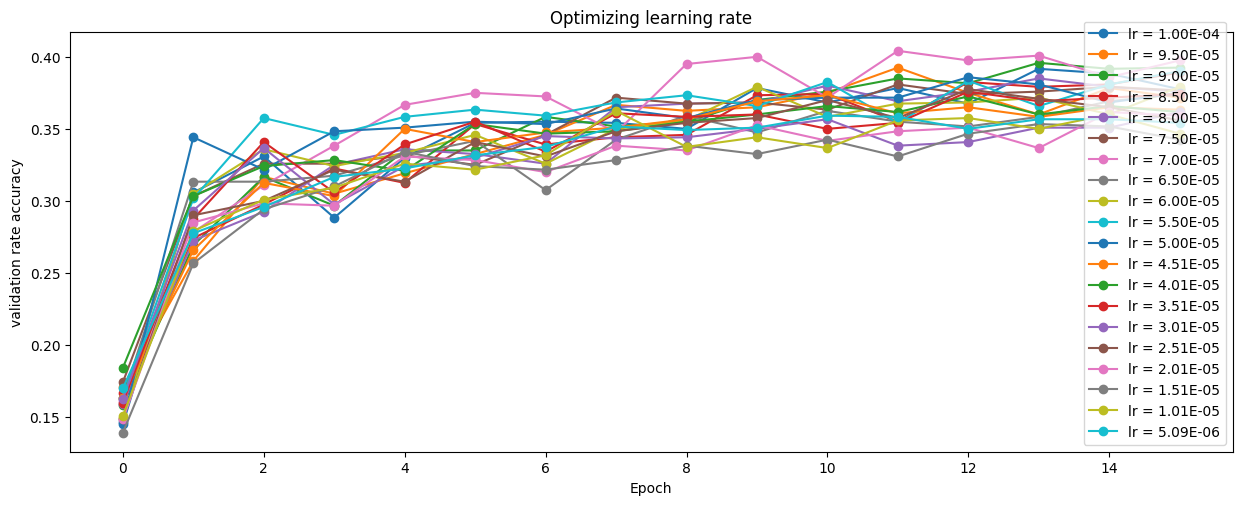
\includegraphics[scale = 0.50]{../src/optimizers/outputs/grid_search/learning_rates.png}}}
  \end{figure}


\item \textbf{Using dropout}\\


\item \textbf{L2 vs dropout}:\\

\item \textbf{Optimizing the topology of the layer}:\\  
  
\item \textbf{How to retrieve our best trained model}:\\
\end{itemize}
  



Now that we had a better idea of the range of the hyperparameters, we launched a random search, optimizing
